%!TEX TS-program = xelatex
%!TEX encoding = UTF-8 Unicode
\documentclass{icis}

\usepackage{graphicx}
\usepackage{xcolor}
\usepackage{tabularx}
\usepackage{booktabs}
\usepackage{array}
\usepackage{ragged2e}
\usepackage{tikz}
\usetikzlibrary{arrows.meta,positioning}
\usepackage{enumitem}
\usepackage{setspace}
\newcolumntype{Y}{>{\RaggedRight\arraybackslash}X}

\title{RISK MANAGEMENT AND IT GOVERNANCE IN THE ADOPTION OF QUANTUM COMPUTING: A CONCEPTUAL MODEL PROPOSAL BASED ON COBIT 5}
\researchtype{Short Paper}
\shorttitle{Quantum IT Governance and Risk Management}
\conference{5th Congress of Corporate Risk Management (CGRC)}

\usepackage[hidelinks]{hyperref}
\addbibresource{references.bib}

% Compact, consistent formatting for the References section
\AtBeginBibliography{%
  \small
  \setlength{\bibhang}{1.2em}
  \setlength{\bibitemsep}{0.32\baselineskip plus 0.05\baselineskip minus 0.05\baselineskip}
  \sloppy
  \hyphenpenalty=10000
  \exhyphenpenalty=10000
}

\begin{document}

\maketitle

\begin{table}[h!]
  \centering
  \LARGE
  \begin{tabularx}{\textwidth}{@{}*2{>{\centering\arraybackslash}X}@{}}
    \textbf{Maria Eduarda Jacinto}        & \textbf{Catharina Moura Moreira} \\
    Chemistry Institute (IQ), University of S\~ao Paulo (USP) & Institute of Mathematics and Computer Science, University of S\~ao Paulo (ICMC/USP) \\
    \\
    \multicolumn{2}{c}{\textbf{Nara Avila Moraes}} \\
    \multicolumn{2}{c}{Physics Institute (IF), University of S\~ao Paulo (USP)} \\
  \end{tabularx}
\end{table}

\begin{abstract}
Quantum computing has emerged as a high-impact, transformative technology with the potential to reshape data-intensive sectors that depend on advanced analytical capacity, such as finance, biotechnology, engineering, logistics, and information security. Although its disruptive potential is widely recognized, corporate adoption remains limited due to significant uncertainties associated with the current era of NISQ (Noisy Intermediate-Scale Quantum) devices, which are characterized by low scalability, high sensitivity to noise, and relevant operational constraints. Recent reports from the Boston Consulting Group (2024) and McKinsey (2024) indicate that organizations understand the need to prepare for this new paradigm, yet still lack structured governance mechanisms, maturity assessment processes, and robust risk management frameworks capable of guiding technological investments in a secure and strategic manner. In response to this scenario, this article proposes a conceptual model that integrates principles of IT governance---particularly those of COBIT 5---with organizational maturity guidelines established by CMMI and MPS.BR, combined with the technical and strategic foundations of quantum computing. The objective is to offer a methodological structure that helps organizations identify internal gaps, assess their readiness for emerging technologies, and make technological decisions with greater predictability. By articulating governance, process maturity, and frontier innovation, the model seeks to reduce information asymmetry, mitigate technological risks, and support business leaders in developing progressive adoption strategies that align innovation with security in a sustainable manner. Thus, this work contributes to advancing discussions on risk management in disruptive technologies and provides a preliminary instrument for future empirical validation.

\emph{\textbf{Keywords:} Corporate IT Governance; Applied Quantum Computing; Technological Risk Assessment; Organizational Process Maturity; COBIT 5; NISQ}
\end{abstract}

\section{Introduction}
The adoption of emerging technologies has always been associated with the need to balance innovation, risk, and responsibility from technical, ethical, and social perspectives. Hoffmann and Flöther (\citeyear{hoffmann2024}) argue that the adoption of AI and quantum computing by businesses must be ethical and cannot be treated merely as an extension of traditional IT. In this context, quantum computing is recognized as an emerging foundational technology with the potential to profoundly reshape sectors that rely heavily on mathematical modeling, simulation, optimization, and the analysis of large volumes of data. At the same time, it creates new normative dilemmas arising from the specific technical characteristics of quantum systems and their distributive impacts. Nevertheless, its incorporation into corporate environments remains constrained by technological uncertainties, particularly in the NISQ era, by information asymmetries between suppliers and decision-makers, and by the absence of consolidated governance guidelines that explicitly integrate ethical principles, accountability criteria, and risk management mechanisms for frontier technologies.

In this context, it becomes increasingly relevant to connect IT governance frameworks such as COBIT 5 with approaches to quantum ethics and Responsible Quantum Technology, which propose incorporating ethical, legal, social, political, and impact (ELSPI) considerations from the early stages of quantum computing research, development, and deployment \parencite{perrier2022,kop2024}. Maturity models such as CMMI and MPS.BR complement this approach by providing criteria for assessing an organization's capacity to absorb complex technologies and implement risk management mechanisms compatible with the specific challenges of quantum architectures and hybrid quantum--classical environments. Accordingly, this study proposes a model that integrates governance, risk management, process maturity, and responsible innovation, providing a structured path for organizations to explore the potential of quantum computing in an ethically oriented manner aligned with sustainable business value creation.

\section{Theoretical Background}
\subsection{IT Governance and COBIT 5}
COBIT 5, developed by ISACA (\citeyear{isaca2012a,isaca2012b,isaca2012c}), is one of the leading international references for IT governance and management. Based on principles such as value delivery, risk optimization, and strategic alignment, the framework establishes processes that are essential to organizational decision-making. Among them are:
\begin{itemize}[leftmargin=*]
    \item EDM02 -- Ensure Benefits Delivery;
    \item APO12 -- Manage Risk;
    \item BAI01 -- Manage Programs and Projects;
    \item MEA01 -- Monitor, Evaluate and Assess Performance and Conformance.
\end{itemize}
These processes are particularly relevant when companies evaluate disruptive technologies, where risk, innovation, and financial return are closely intertwined.

\subsection{Quantum Computing and Its Challenges}
Quantum computing has been identified as one of the most promising technologies of the past decade, but its practical applicability remains limited by the immaturity of currently available systems. Preskill (\citeyear{preskill2018}) characterizes the present period as the era of NISQ (Noisy Intermediate-Scale Quantum) devices, in which quantum computers operate with a limited number of qubits, high susceptibility to noise, and no robust error-correction schemes. These characteristics make system behavior unstable and difficult to predict for applications requiring reliability and reproducibility in corporate environments. In addition, the performance of quantum algorithms depends directly on factors such as qubit coherence, hardware topology, noise rates, and gate fidelity, all of which vary significantly across providers and platforms.

Despite these limitations, recent reports from consulting firms \parencite{bcg2024,mckinsey2024} indicate that several areas may offer significant potential benefits, particularly in contexts where classical computing begins to encounter physical or mathematical scaling limits. The most promising areas include:
\begin{itemize}[leftmargin=*]
    \item \textbf{Bioinformatics and drug development:} quantum simulation may accelerate the modeling of molecular interactions, enable more accurate predictions of chemical structures, and shorten drug-discovery cycles.
    \item \textbf{Advanced engineering and physical simulation:} quantum algorithms may be suitable for highly complex problems such as fluid dynamics, materials simulation, structural optimization, and thermodynamic processes that are difficult to model classically.
    \item \textbf{Finance and risk modeling:} quantum techniques may improve portfolio optimization, risk analysis, derivatives pricing, and high-dimensional Monte Carlo simulations.
    \item \textbf{Logistics and combinatorial problems:} variational algorithms and hybrid heuristics may improve routing, resource allocation, and production sequencing in scenarios with high combinatorial complexity.
    \item \textbf{Security and post-quantum cryptography:} although the threat to cryptographic systems remains prospective, organizations need to prepare for the regulatory and strategic transitions required by emerging post-quantum security standards.
\end{itemize}

Nevertheless, despite this sectoral potential, most companies still lack sufficient organizational maturity, technical infrastructure, or internal expertise to conduct risk assessments or implement quantum pilots safely and efficiently. The gap between the theoretical potential of quantum computing and organizations' practical execution capacity reinforces the need for formal governance structures and systematic technology-readiness assessment processes capable of aligning quantum initiatives with corporate strategy, risk management, and existing process-maturity levels.

\subsection{Maturity Models: CMMI and MPS.BR}
The adoption of emerging technologies requires organizations to maintain stable, predictable, and well-documented internal processes. The CMMI (Capability Maturity Model Integration), developed by the Software Engineering Institute, and MPS.BR (Brazilian Software Process Improvement), maintained by Softex, provide established references for evaluating an organization's ability to develop, implement, and sustain complex technological solutions \parencite{sei2010,softex2022}. Both are based on the premise that innovation generates value consistently only when supported by structured processes, clear responsibilities, control mechanisms, and formal continuous-improvement cycles.

Table~\ref{tab:maturity} summarizes the main structural components of process maturity.
\begin{table}[htbp]
\centering
\caption{Structural Components of Process Maturity}
\label{tab:maturity}
\begin{tabularx}{\textwidth}{>{\bfseries}p{0.27\textwidth}Y}
\toprule
Element & Description \\
\midrule
Process standardization & Clear definition of responsibilities, workflows, and artifacts, avoiding improvisation that could compromise highly complex projects. \\
Management capability & Formal mechanisms for planning, monitoring, and control, including performance metrics and critical-analysis tools. \\
Predictability & Reduction of process variability, allowing expected results to be projected and monitored. \\
Documentation and measurement & Systematic recording of activities and indicators so that future decisions are based on evidence rather than intuition alone. \\
Continuous improvement & Establishment of iterative refinement cycles, ensuring that the organization evolves over time and can absorb increasingly challenging technologies. \\
\bottomrule
\end{tabularx}
\begin{flushright}\small Source: The Authors, 2025.\end{flushright}
\end{table}

When integrated with COBIT 5, these maturity models strengthen an organization's ability to align risk management, governance, and technology strategy. COBIT 5 provides the governance structure, including processes, controls, and strategic-alignment mechanisms, while CMMI and MPS.BR make it possible to assess the operational capacity that will support the adoption of emerging technologies. This combination creates a more robust basis for decision-making, allowing quantum-computing initiatives to be classified according to multiple criteria, such as technical readiness, internal maturity, associated risks, potential impact, and strategic alignment. As a result, companies can avoid premature decisions or high-risk investments without adequate technical support while building a clear view of the capabilities they need to develop in order to move toward the safe and gradual adoption of quantum computing.

The integration of NISQ-era quantum computing, COBIT 5-based IT governance, process-maturity models, and technology readiness levels is summarized in Figure~\ref{fig:model}.

\begin{figure}[htbp]
\centering
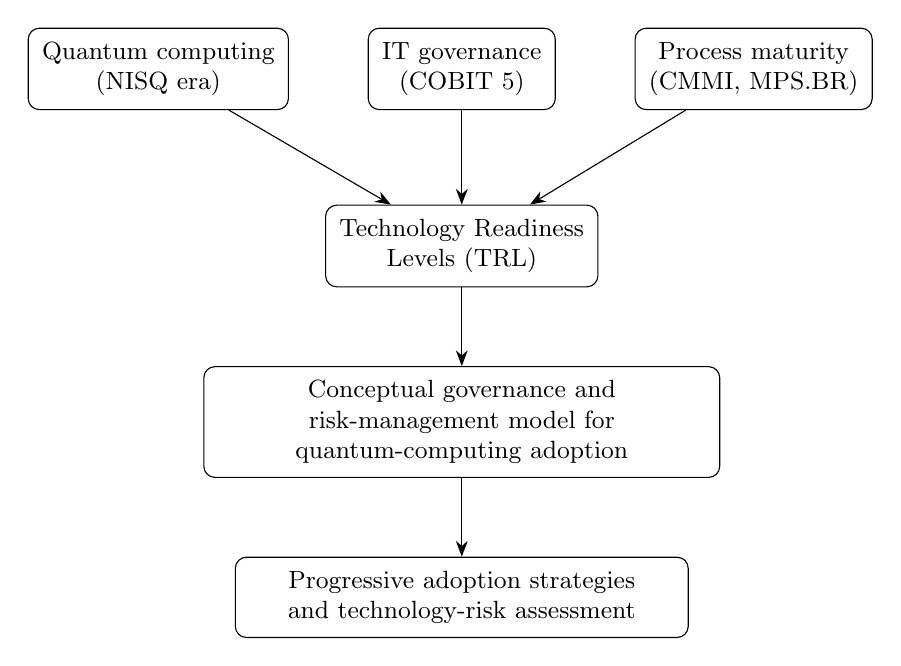
\begin{tikzpicture}[node distance=1.0cm and 1.0cm, every node/.style={draw, rounded corners, align=center, font=\small, inner sep=5pt}, >={Stealth[length=2mm]}]
\node (qc) {Quantum computing\\(NISQ era)};
\node[right=of qc] (gov) {IT governance\\(COBIT 5)};
\node[right=of gov] (mat) {Process maturity\\(CMMI, MPS.BR)};
\node[below=1.2cm of gov] (trl) {Technology Readiness\\Levels (TRL)};
\node[below=of trl, text width=6.2cm] (model) {Conceptual governance and risk-management model for quantum-computing adoption};
\node[below=of model, text width=5.4cm] (strategy) {Progressive adoption strategies and technology-risk assessment};
\draw[->] (qc) -- (trl); \draw[->] (gov) -- (trl); \draw[->] (mat) -- (trl);
\draw[->] (trl) -- (model); \draw[->] (model) -- (strategy);
\end{tikzpicture}
\caption{Integrative conceptual model of quantum computing, IT governance, and process maturity.}
\label{fig:model}
\begin{flushright}\small Source: The Authors, 2025.\end{flushright}
\end{figure}

\section{Methodology}
This research adopts a qualitative, exploratory, and theory-building approach appropriate to the objective of developing a conceptual governance and risk-management model for the adoption of quantum technologies in organizational environments. Because quantum computing remains at a limited stage of maturity, characterized by the NISQ era, and governance practices in this domain are still incipient, there are currently no broadly consolidated models that enable large-scale empirical assessment. In this context, the methodology prioritizes systematic theoretical construction supported by specialized sources and internationally recognized frameworks.

\subsection{Research Design}
The study is characterized as qualitative exploratory research whose central purpose is to deepen understanding of the challenges, risks, and governance requirements associated with corporate adoption of quantum computing. This design is justified by the complexity of the phenomenon under analysis and by the absence of technical and methodological standardization in the sector, which makes traditional experimental or quantitative approaches unsuitable at this stage.

The research also has a theory-building character because it seeks to integrate conceptual elements from three distinct domains---quantum computing, IT governance, and maturity models---with the objective of formulating a model that supports decision-making on quantum-computing adoption while considering risks, organizational capabilities, and maturity stage.

\subsection{Methodological Procedures}
The research was developed in three main stages, articulated sequentially and iteratively.

\paragraph{Stage 1 -- Review of specialized literature.}
A systematic review of technical, scientific, and institutional literature was conducted. It covered scientific articles on quantum computing, with emphasis on the NISQ era \parencite{preskill2018}; strategic consulting reports, including BCG and McKinsey \parencite{bcg2024,mckinsey2024}; official COBIT 5 documentation \parencite{isaca2012a,isaca2012b,isaca2012c}; international maturity models, including CMMI and MPS.BR \parencite{sei2010,softex2022}; and specialized publications addressing governance, technological risks, and disruptive innovation. This review made it possible to identify theoretical gaps, conceptual convergences, and structural elements relevant to the proposed model.

\paragraph{Stage 2 -- Conceptual mapping and risk categorization.}
Based on the reviewed literature, risk categories associated with the adoption of quantum technologies were mapped, as summarized in Table~\ref{tab:risks}.

\begin{table}[htbp]
\centering
\caption{Risk Categories Associated with the Adoption of Quantum Technologies}
\label{tab:risks}
\begin{tabularx}{\textwidth}{>{\bfseries}p{0.33\textwidth}Y}
\toprule
Risk Category & Description \\
\midrule
Technological risks & Related to the limitations of NISQ devices. \\
Operational risks & Involve hybrid integration and technical training. \\
Strategic risks & Associated with alignment between innovation and corporate objectives. \\
Regulatory and security risks & Especially related to post-quantum cryptography. \\
Financial risks & Refer to uncertainty regarding return on investment (ROI). \\
\bottomrule
\end{tabularx}
\begin{flushright}\small Source: The Authors, 2025.\end{flushright}
\end{table}

In parallel, the COBIT 5 processes directly related to these risks were identified, notably EDM02 (Ensure Benefits Delivery), APO12 (Manage Risk), BAI01 (Manage Programs and Projects), and MEA01 (Monitor, Evaluate and Assess Performance and Conformance). The categorization was conducted through thematic analysis, enabling relationships to be established between the specific challenges of quantum computing and governance practices already consolidated in corporate environments.

In addition to Table~\ref{tab:risks}, the risk categories are represented schematically in Figure~\ref{fig:risks}, highlighting the centrality of corporate quantum-computing adoption and the different types of exposure associated with this process.

\begin{figure}[htbp]
\centering
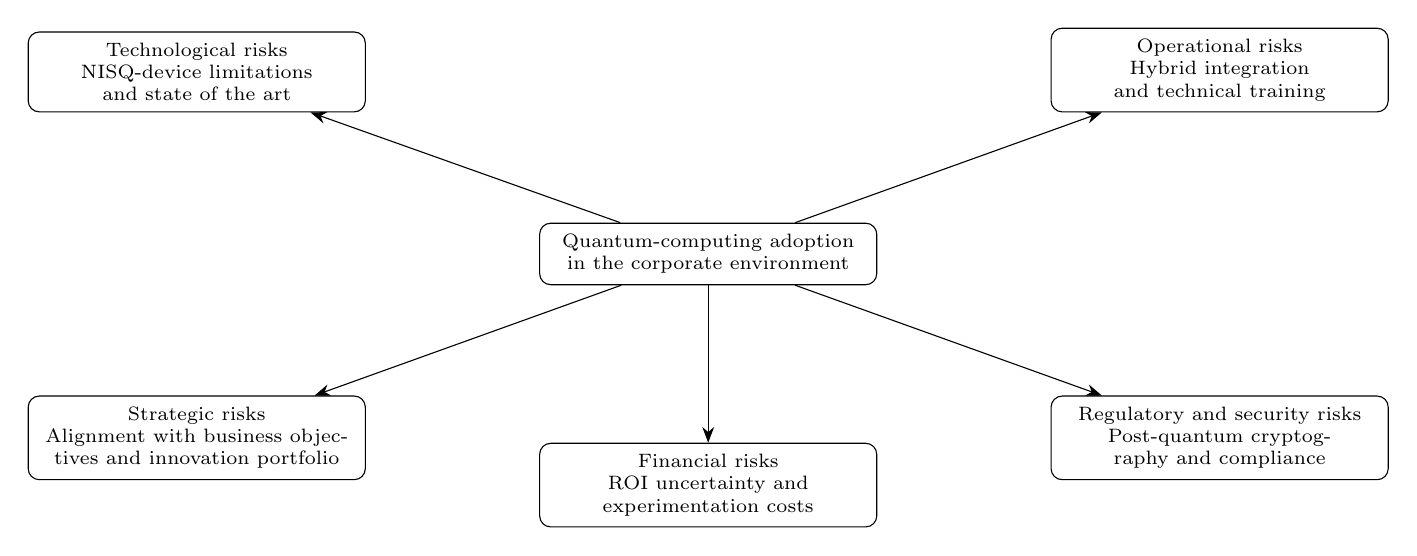
\begin{tikzpicture}[every node/.style={draw, rounded corners, align=center, font=\scriptsize, inner sep=4pt}, >={Stealth[length=2mm]}]
\node[text width=4cm] (center) {Quantum-computing adoption\\in the corporate environment};
\node[above left=1.4cm and 2.2cm of center, text width=4cm] (tech) {Technological risks\\NISQ-device limitations and state of the art};
\node[above right=1.4cm and 2.2cm of center, text width=4cm] (op) {Operational risks\\Hybrid integration and technical training};
\node[below left=1.4cm and 2.2cm of center, text width=4cm] (strat) {Strategic risks\\Alignment with business objectives and innovation portfolio};
\node[below right=1.4cm and 2.2cm of center, text width=4cm] (reg) {Regulatory and security risks\\Post-quantum cryptography and compliance};
\node[below=2.0cm of center, text width=4cm] (fin) {Financial risks\\ROI uncertainty and experimentation costs};
\draw[->] (center)--(tech); \draw[->] (center)--(op); \draw[->] (center)--(strat); \draw[->] (center)--(reg); \draw[->] (center)--(fin);
\end{tikzpicture}
\caption{Risk categories associated with the adoption of quantum computing in organizations.}
\label{fig:risks}
\begin{flushright}\small Source: The Authors, 2025.\end{flushright}
\end{figure}

\paragraph{Stage 3 -- Construction of the integrative conceptual model.}
Using the identified theoretical elements, an integrated conceptual model was developed that articulates:
\begin{enumerate}[leftmargin=*]
    \item the limitations and potential of quantum computing in the NISQ era;
    \item COBIT 5 principles and processes applicable to technology decision-making;
    \item maturity requirements defined by CMMI and MPS.BR; and
    \item an incremental assessment logic based on Technology Readiness Levels (TRL).
\end{enumerate}

The model was constructed according to a deductive logic, connecting governance, organizational maturity, and technology readiness to generate a coherent framework applicable to the corporate context. Conceptual validation was conducted through theoretical triangulation by comparing the model's components with similar frameworks described in the international literature on innovation, technology management, and emerging-technology adoption.

The three stages are summarized in Figure~\ref{fig:method}.
\begin{figure}[htbp]
\centering
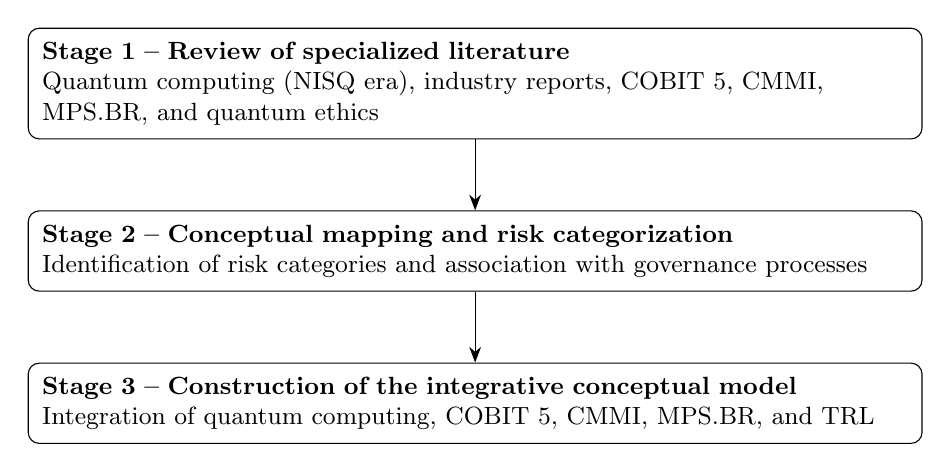
\begin{tikzpicture}[node distance=.9cm, every node/.style={draw, rounded corners, align=left, font=\small, text width=11cm, inner sep=5pt}, >={Stealth[length=2mm]}]
\node (s1) {\textbf{Stage 1 -- Review of specialized literature}\\Quantum computing (NISQ era), industry reports, COBIT 5, CMMI, MPS.BR, and quantum ethics};
\node[below=of s1] (s2) {\textbf{Stage 2 -- Conceptual mapping and risk categorization}\\Identification of risk categories and association with governance processes};
\node[below=of s2] (s3) {\textbf{Stage 3 -- Construction of the integrative conceptual model}\\Integration of quantum computing, COBIT 5, CMMI, MPS.BR, and TRL};
\draw[->] (s1)--(s2); \draw[->] (s2)--(s3);
\end{tikzpicture}
\caption{Stages of the theory-building methodology adopted in the research.}
\label{fig:method}
\begin{flushright}\small Source: The Authors, 2025.\end{flushright}
\end{figure}

\subsection{Methodological Rationale}
The choice of a theory-building approach is based on two main factors. First, the absence of consolidated structures for quantum-computing governance makes large-scale empirical studies premature, particularly in corporate environments that still operate predominantly in an exploratory phase. Second, the interdisciplinary complexity of the topic requires the integration of knowledge from computer science, organizational engineering, and corporate governance, reinforcing the suitability of a strategy oriented toward conceptual construction and synthesis of reference frameworks.

Accordingly, the adopted methodology makes it possible to construct a rigorous, well-founded, and methodologically traceable model, providing a basis for future applied research, case studies, and empirical investigations aimed at testing and refining the proposal.

\subsection{Methodological Limitations}
The limitations of this research include the absence of empirical validation, resulting from the still-incipient maturity of the quantum industry and the lack of broadly consolidated corporate applications; dependence on technical and prospective literature, whose dynamic nature makes it susceptible to rapid change as technologies and markets evolve; and limitations inherent to conceptual models, which may require sector-specific adaptations or adjustments according to the maturity level of the organizations that apply them. Nevertheless, these limitations are consistent with the current stage of development of the field and reinforce the relevance of the proposed model as a preliminary instrument for guiding more robust future research, applied case studies, and empirical validations that can strengthen and expand its applicability.

\section{Analysis of Results}
The analysis of the results obtained from applying the proposed methodology indicates that integrating emerging quantum computing, governance frameworks, and organizational maturity models provides a structured path for assessing and mitigating technological risks. The findings help clarify not only the potential applications of quantum computing but, above all, the challenges associated with its adoption from the perspectives of corporate governance and risk management.

\subsection{Mapping Governance and Maturity Gaps}
The comparative assessment of COBIT 5 principles and the maturity levels of the CMMI and MPS.BR models indicates that most of the organizations analyzed, represented here by the ``Cautious Executive'' persona, are at intermediate maturity stages, close to levels 2 and 3. These levels characterize companies that are capable of managing processes but still have low predictability and insufficient documentation to support high-impact technological experimentation. This situation confirms the concerns captured by the qualitative instruments used to characterize the Cautious Executive, including concern about risky investments, strong information asymmetry, and the absence of formal assessment mechanisms.

Cross-referencing the risk-matrix data with COBIT 5 principles revealed specific weaknesses in three central processes:
\begin{itemize}[leftmargin=*]
    \item \textbf{APO12 -- Manage Risk:} absence of quantifiable criteria for measuring emerging technological risks;
    \item \textbf{BAI03 -- Manage Solutions Identification and Build:} limited internal capacity for prototyping and structured testing;
    \item \textbf{MEA01 -- Monitor, Evaluate and Assess Performance and Conformance:} lack of robust indicators for evaluating the return from innovative technologies.
\end{itemize}
These gaps constitute significant barriers to the adoption of quantum-computing solutions, including Quantum Machine Learning applications, because they limit an organization's ability to test, learn from, and scale initiatives in a controlled manner.

\subsection{Results from Applying the Technological Risk-Assessment Framework}
Applying the technological risk matrix developed in the methodology identified three main critical dimensions. The first concerns technical risks associated with the immaturity of quantum technology in the NISQ era, characterized by devices with a limited number of qubits, high susceptibility to noise, and the absence of robust error-correction schemes \parencite{preskill2018}. These factors translate into operational instability, limited algorithm scalability, and dependence on highly specialized teams. Taken together, they reinforce the assessment presented in strategic consulting reports \parencite{bcg2024,mckinsey2024}, according to which progress in corporate quantum-computing adoption will depend on the existence of more robust and rigorous governance structures.

The second dimension encompasses organizational risks related to internal maturity and technological integration capacity. These risks manifest in the lack of process standardization, the presence of legacy IT environments with limited compatibility with hybrid classical--quantum workflows, and the absence of formal mechanisms for accountability and funding of innovative initiatives. These limitations indicate that governance occupies a central position in the technology-incorporation process because it conditions the organization's ability to experiment with, evaluate, and adjust highly complex projects.

The third dimension concerns strategic risks, regarded in the source study as particularly sensitive. These include investments without demonstrated returns, difficulties in technical communication between business and IT areas, and perceptions of inflated expectations and uncertainty regarding the practical applicability of quantum computing. These factors directly influence the decision-making process of executives responsible for innovation, reinforcing the cautious stance represented by the persona.

\subsection{Feasibility of Practical Applications in Strategic Sectors}
The analysis of quantum-computing applicability in sectors such as pharmaceuticals, engineering, finance, and logistics---frequently highlighted in the literature and market reports as high-potential areas---shows that possible gains depend on two structural variables. The first is the availability of structured and standardized data, consistent with the process-maturity principles advocated by CMMI and MPS.BR. The second is the existence of consistent technology-governance mechanisms aligned with the planning, risk-management, and monitoring guidelines proposed by COBIT 5.

Without these elements, transitioning from experimentation to value generation at scale becomes difficult, even in scenarios in which quantum algorithms present theoretical superiority. The sectoral analysis indicates that applicability in bioinformatics and drug development is high but depends on highly regulated environments and strong control over sensitive data. In engineering and physical simulation, potential gains are significant, although they require sophisticated hybrid infrastructure and specialized technical teams. In the financial sector, greater maturity in governance and risk management supports exploratory initiatives, but caution remains because of high costs and technological uncertainties. In logistics, the potential associated with solving complex combinatorial problems is high, yet operational obstacles, integration limitations, and heterogeneous maturity among supply-chain actors continue to hinder immediate adoption.

\subsection{Summary of Results}
The main conclusion of this stage is that quantum-computing adoption does not depend exclusively on technological evolution; it also requires a robust governance framework, process maturity, and clear risk-assessment metrics. In practice, these elements emerge as the principal limiting variables identified in the study. The results indicate that organizations with intermediate maturity levels and limited integration of governance practices will face significant difficulties in advancing quantum initiatives safely and sustainably.

The findings also indicate that established frameworks such as COBIT 5, CMMI, and MPS.BR should not be treated as optional elements within the proposed model, but as requirements for guiding strategic decisions, mitigating risks, and ensuring predictability in emerging-technology projects. Thus, although quantum computing has substantial transformative potential across multiple sectors, its practical applicability will depend on alignment among strategy, risk management, and organizational processes, consistent with the classical literature on IT governance and management.

This analysis therefore reinforces the relevance of the proposed conceptual model and provides a basis for the recommendations presented in the conclusions, particularly the need to strengthen governance structures, increase process maturity, and improve technology-readiness assessment before investment decisions involving quantum computing.

\section{Conclusions}
The results of this study indicate that corporate adoption of quantum technologies, particularly in the context of NISQ devices, depends less on isolated technical progress than on organizational capacity to structure processes, mitigate risks, and establish formal governance mechanisms. The integrated analysis of COBIT 5, CMMI, and MPS.BR shows that, although quantum computing has substantial potential impact in sectors such as bioinformatics, engineering, finance, and logistics, its practical incorporation remains constrained by weaknesses in standardization, measurement, documentation, and operational predictability. In this sense, the main contribution of this work is the formulation of a conceptual model capable of supporting technological risk assessment and decision-making, translating quantum potential into measurable business value aligned with organizations' strategic needs.

The findings also indicate that many companies remain at intermediate levels of organizational maturity, which restricts the safe and effective adoption of emerging technologies. This scenario reinforces the importance of greater integration between technical and strategic areas, fostering an environment in which decisions about quantum technologies are based not only on technical factors but also on governance criteria, operational capacity, and strategic alignment. The proposed model serves as a structured reference for identifying internal gaps, guiding investment prioritization, and establishing progressive pathways for quantum-solution adoption, thereby reducing information asymmetries and increasing the predictability of innovation initiatives.

Finally, the limitations of this study---associated with the still-incipient maturity of the quantum industry, dependence on technical and prospective literature, and the inherent constraints of conceptual models---point to the need for future empirical research to validate and improve the model in real organizational contexts. Subsequent investigations may deepen understanding of the relationship among governance, corporate strategy, and disruptive technologies, contributing to the construction of more robust frameworks applicable to organizations seeking to integrate quantum computing safely, gradually, and sustainably.

\printbibliography

\end{document}
